\documentclass[twoside]{book}

% Packages required by doxygen
\usepackage{calc}
\usepackage{doxygen}
\usepackage{graphicx}
\usepackage[utf8]{inputenc}
\usepackage{makeidx}
\usepackage{multicol}
\usepackage{multirow}
\usepackage{textcomp}
\usepackage[table]{xcolor}

% Font selection
\usepackage[T1]{fontenc}
\usepackage{mathptmx}
\usepackage[scaled=.90]{helvet}
\usepackage{courier}
\usepackage{amssymb}
\usepackage{sectsty}
\renewcommand{\familydefault}{\sfdefault}
\allsectionsfont{%
  \fontseries{bc}\selectfont%
  \color{darkgray}%
}
\renewcommand{\DoxyLabelFont}{%
  \fontseries{bc}\selectfont%
  \color{darkgray}%
}

% Page & text layout
\usepackage{geometry}
\geometry{%
  a4paper,%
  top=2.5cm,%
  bottom=2.5cm,%
  left=2.5cm,%
  right=2.5cm%
}
\tolerance=750
\hfuzz=15pt
\hbadness=750
\setlength{\emergencystretch}{15pt}
\setlength{\parindent}{0cm}
\setlength{\parskip}{0.2cm}
\makeatletter
\renewcommand{\paragraph}{%
  \@startsection{paragraph}{4}{0ex}{-1.0ex}{1.0ex}{%
    \normalfont\normalsize\bfseries\SS@parafont%
  }%
}
\renewcommand{\subparagraph}{%
  \@startsection{subparagraph}{5}{0ex}{-1.0ex}{1.0ex}{%
    \normalfont\normalsize\bfseries\SS@subparafont%
  }%
}
\makeatother

% Headers & footers
\usepackage{fancyhdr}
\pagestyle{fancyplain}
\fancyhead[LE]{\fancyplain{}{\bfseries\thepage}}
\fancyhead[CE]{\fancyplain{}{}}
\fancyhead[RE]{\fancyplain{}{\bfseries\leftmark}}
\fancyhead[LO]{\fancyplain{}{\bfseries\rightmark}}
\fancyhead[CO]{\fancyplain{}{}}
\fancyhead[RO]{\fancyplain{}{\bfseries\thepage}}
\fancyfoot[LE]{\fancyplain{}{}}
\fancyfoot[CE]{\fancyplain{}{}}
\fancyfoot[RE]{\fancyplain{}{\bfseries\scriptsize Generated on Fri Nov 28 2014 10\-:03\-:06 for My Project by Doxygen }}
\fancyfoot[LO]{\fancyplain{}{\bfseries\scriptsize Generated on Fri Nov 28 2014 10\-:03\-:06 for My Project by Doxygen }}
\fancyfoot[CO]{\fancyplain{}{}}
\fancyfoot[RO]{\fancyplain{}{}}
\renewcommand{\footrulewidth}{0.4pt}
\renewcommand{\chaptermark}[1]{%
  \markboth{#1}{}%
}
\renewcommand{\sectionmark}[1]{%
  \markright{\thesection\ #1}%
}

% Indices & bibliography
\usepackage{natbib}
\usepackage[titles]{tocloft}
\setcounter{tocdepth}{3}
\setcounter{secnumdepth}{5}
\makeindex

% Hyperlinks (required, but should be loaded last)
\usepackage{ifpdf}
\ifpdf
  \usepackage[pdftex,pagebackref=true]{hyperref}
\else
  \usepackage[ps2pdf,pagebackref=true]{hyperref}
\fi
\hypersetup{%
  colorlinks=true,%
  linkcolor=blue,%
  citecolor=blue,%
  unicode%
}

% Custom commands
\newcommand{\clearemptydoublepage}{%
  \newpage{\pagestyle{empty}\cleardoublepage}%
}


%===== C O N T E N T S =====

\begin{document}

% Titlepage & ToC
\hypersetup{pageanchor=false}
\pagenumbering{roman}
\begin{titlepage}
\vspace*{7cm}
\begin{center}%
{\Large My Project }\\
\vspace*{1cm}
{\large Generated by Doxygen 1.8.6}\\
\vspace*{0.5cm}
{\small Fri Nov 28 2014 10:03:06}\\
\end{center}
\end{titlepage}
\clearemptydoublepage
\tableofcontents
\clearemptydoublepage
\pagenumbering{arabic}
\hypersetup{pageanchor=true}

%--- Begin generated contents ---
\chapter{Namespace Index}
\section{Namespace List}
Here is a list of all documented namespaces with brief descriptions\-:\begin{DoxyCompactList}
\item\contentsline{section}{\hyperlink{namespaceliftedLP__glpk}{lifted\-L\-P\-\_\-glpk} \\*T\-O\-D\-O }{\pageref{namespaceliftedLP__glpk}}{}
\item\contentsline{section}{\hyperlink{namespacesymLPExperiments}{sym\-L\-P\-Experiments} \\*Modul, which acts as a framework for the actual lifting }{\pageref{namespacesymLPExperiments}}{}
\end{DoxyCompactList}

\chapter{Hierarchical Index}
\section{Class Hierarchy}
This inheritance list is sorted roughly, but not completely, alphabetically\-:\begin{DoxyCompactList}
\item \contentsline{section}{amorph\-\_\-graph}{\pageref{structamorph__graph}}{}
\item binary\-\_\-function\begin{DoxyCompactList}
\item \contentsline{section}{iequal\-\_\-to}{\pageref{structiequal__to}}{}
\end{DoxyCompactList}
\item \contentsline{section}{coloring}{\pageref{structcoloring}}{}
\item \contentsline{section}{dimacs\-\_\-info}{\pageref{structdimacs__info}}{}
\item \contentsline{section}{option}{\pageref{structoption}}{}
\item \contentsline{section}{saucy}{\pageref{structsaucy}}{}
\item \contentsline{section}{saucy\-\_\-graph}{\pageref{structsaucy__graph}}{}
\item \contentsline{section}{saucy\-\_\-stats}{\pageref{structsaucy__stats}}{}
\item \contentsline{section}{sorter$<$ T $>$}{\pageref{classsorter}}{}
\item unary\-\_\-function\begin{DoxyCompactList}
\item \contentsline{section}{ihash}{\pageref{structihash}}{}
\end{DoxyCompactList}
\end{DoxyCompactList}

\chapter{Class Index}
\section{Class List}
Here are the classes, structs, unions and interfaces with brief descriptions\-:\begin{DoxyCompactList}
\item\contentsline{section}{\hyperlink{structamorph__graph}{amorph\-\_\-graph} }{\pageref{structamorph__graph}}{}
\item\contentsline{section}{\hyperlink{structcoloring}{coloring} }{\pageref{structcoloring}}{}
\item\contentsline{section}{\hyperlink{structdimacs__info}{dimacs\-\_\-info} }{\pageref{structdimacs__info}}{}
\item\contentsline{section}{\hyperlink{structiequal__to}{iequal\-\_\-to} }{\pageref{structiequal__to}}{}
\item\contentsline{section}{\hyperlink{structihash}{ihash} }{\pageref{structihash}}{}
\item\contentsline{section}{\hyperlink{structoption}{option} }{\pageref{structoption}}{}
\item\contentsline{section}{\hyperlink{structsaucy}{saucy} }{\pageref{structsaucy}}{}
\item\contentsline{section}{\hyperlink{structsaucy__graph}{saucy\-\_\-graph} }{\pageref{structsaucy__graph}}{}
\item\contentsline{section}{\hyperlink{structsaucy__stats}{saucy\-\_\-stats} }{\pageref{structsaucy__stats}}{}
\item\contentsline{section}{\hyperlink{classsorter}{sorter$<$ T $>$} }{\pageref{classsorter}}{}
\end{DoxyCompactList}

\chapter{Namespace Documentation}
\hypertarget{namespacesymLPExperiments}{\section{sym\-L\-P\-Experiments Namespace Reference}
\label{namespacesymLPExperiments}\index{sym\-L\-P\-Experiments@{sym\-L\-P\-Experiments}}
}


Documentation for this module.  


\subsection*{Functions}
\begin{DoxyCompactItemize}
\item 
def \hyperlink{namespacesymLPExperiments_a00f49f67a2a2d9e675d6f392a28c6d21}{extract\-\_\-matrix}
\begin{DoxyCompactList}\small\item\em Extracts a coordinate matrix from a given n-\/dimensional array Creates a coordinate matrix for the given lpmatrix, by extracting necessary values from the given lpmatrix. \end{DoxyCompactList}\item 
def \hyperlink{namespacesymLPExperiments_a13db8437b54c2d6e412fdca6beebcd73}{load\-Nsolve}
\begin{DoxyCompactList}\small\item\em Loads and solves a given L\-P by lifting the data and then solving it-\/. \end{DoxyCompactList}\item 
def \hyperlink{namespacesymLPExperiments_aac02ec1af252db0b5351036a4725aa22}{load\-Nsolve\-C\-V\-X}
\begin{DoxyCompactList}\small\item\em Solves a given L\-P file by using cvxopt as a method to generate the matrix and glpk to solve it. \end{DoxyCompactList}\item 
def \hyperlink{namespacesymLPExperiments_a0b36c729a222467b8abb13726eeee5f5}{runbatch}
\begin{DoxyCompactList}\small\item\em Iterates over every file specified in the main method. \end{DoxyCompactList}\end{DoxyCompactItemize}
\subsection*{Variables}
\begin{DoxyCompactItemize}
\item 
\hypertarget{namespacesymLPExperiments_a9a922fb530cc4e5f4b3815131fa3c371}{int {\bfseries U\-P\-P\-E\-R} = 3}\label{namespacesymLPExperiments_a9a922fb530cc4e5f4b3815131fa3c371}

\item 
\hypertarget{namespacesymLPExperiments_a59472bb37d81ca8001d5cc3353cf4eaa}{int {\bfseries L\-O\-W\-E\-R} = 2}\label{namespacesymLPExperiments_a59472bb37d81ca8001d5cc3353cf4eaa}

\item 
\hypertarget{namespacesymLPExperiments_a46b8d304e13a7c4130a3188af48eb75f}{int {\bfseries E\-Q\-U\-A\-L} = 5}\label{namespacesymLPExperiments_a46b8d304e13a7c4130a3188af48eb75f}

\item 
\hypertarget{namespacesymLPExperiments_a28e15d061ce80b2268c38cf230c47234}{int {\bfseries U\-N\-B\-O\-U\-N\-D} = 1}\label{namespacesymLPExperiments_a28e15d061ce80b2268c38cf230c47234}

\item 
\hypertarget{namespacesymLPExperiments_af086c1b10d5e4ab2988e689c83bf3f2b}{int {\bfseries G\-E\-O\-M\-M\-E\-A\-N} = 6}\label{namespacesymLPExperiments_af086c1b10d5e4ab2988e689c83bf3f2b}

\item 
\hypertarget{namespacesymLPExperiments_a973f0d69838ed63d09a2d13b5eb5f93a}{int {\bfseries E\-Q\-U\-I\-L\-I\-B} = 7}\label{namespacesymLPExperiments_a973f0d69838ed63d09a2d13b5eb5f93a}

\item 
\hypertarget{namespacesymLPExperiments_a6680909d6fdcc093706c541e3e3295ec}{int {\bfseries L\-P} = 1}\label{namespacesymLPExperiments_a6680909d6fdcc093706c541e3e3295ec}

\item 
\hypertarget{namespacesymLPExperiments_ae4e28dbe2606236884d4f5968b2784b6}{int {\bfseries M\-T\-S} = 0}\label{namespacesymLPExperiments_ae4e28dbe2606236884d4f5968b2784b6}

\end{DoxyCompactItemize}


\subsection{Detailed Description}
Documentation for this module. This module retrieves L\-Ps from specified files and provides the necessary interface to solve given L\-Ps. Calculation and Computation is done in the C/\-C++ core, where most of the work is done. 

\subsection{Function Documentation}
\hypertarget{namespacesymLPExperiments_a00f49f67a2a2d9e675d6f392a28c6d21}{\index{sym\-L\-P\-Experiments@{sym\-L\-P\-Experiments}!extract\-\_\-matrix@{extract\-\_\-matrix}}
\index{extract\-\_\-matrix@{extract\-\_\-matrix}!symLPExperiments@{sym\-L\-P\-Experiments}}
\subsubsection[{extract\-\_\-matrix}]{\setlength{\rightskip}{0pt plus 5cm}def sym\-L\-P\-Experiments.\-extract\-\_\-matrix (
\begin{DoxyParamCaption}
\item[{}]{lpmatrix}
\end{DoxyParamCaption}
)}}\label{namespacesymLPExperiments_a00f49f67a2a2d9e675d6f392a28c6d21}


Extracts a coordinate matrix from a given n-\/dimensional array Creates a coordinate matrix for the given lpmatrix, by extracting necessary values from the given lpmatrix. 


\begin{DoxyParams}{Parameters}
{\em lpmatrix} & The four dimensional array with column and row coordinates in the first two rows and data in the third row \\
\hline
\end{DoxyParams}
\hypertarget{namespacesymLPExperiments_a13db8437b54c2d6e412fdca6beebcd73}{\index{sym\-L\-P\-Experiments@{sym\-L\-P\-Experiments}!load\-Nsolve@{load\-Nsolve}}
\index{load\-Nsolve@{load\-Nsolve}!symLPExperiments@{sym\-L\-P\-Experiments}}
\subsubsection[{load\-Nsolve}]{\setlength{\rightskip}{0pt plus 5cm}def sym\-L\-P\-Experiments.\-load\-Nsolve (
\begin{DoxyParamCaption}
\item[{}]{fname, }
\item[{}]{scaled, }
\item[{}]{ftype}
\end{DoxyParamCaption}
)}}\label{namespacesymLPExperiments_a13db8437b54c2d6e412fdca6beebcd73}


Loads and solves a given L\-P by lifting the data and then solving it-\/. 


\begin{DoxyParams}{Parameters}
{\em fname} & The name of a given file, which contains the L\-P \\
\hline
{\em scaled} & An integer value, which indicates a scaling/scaled L\-P (?) \\
\hline
{\em ftype} & The type of the given problem (mostly L\-Ps) \\
\hline
\end{DoxyParams}
\hypertarget{namespacesymLPExperiments_aac02ec1af252db0b5351036a4725aa22}{\index{sym\-L\-P\-Experiments@{sym\-L\-P\-Experiments}!load\-Nsolve\-C\-V\-X@{load\-Nsolve\-C\-V\-X}}
\index{load\-Nsolve\-C\-V\-X@{load\-Nsolve\-C\-V\-X}!symLPExperiments@{sym\-L\-P\-Experiments}}
\subsubsection[{load\-Nsolve\-C\-V\-X}]{\setlength{\rightskip}{0pt plus 5cm}def sym\-L\-P\-Experiments.\-load\-Nsolve\-C\-V\-X (
\begin{DoxyParamCaption}
\item[{}]{fname, }
\item[{}]{scaled, }
\item[{}]{ftype}
\end{DoxyParamCaption}
)}}\label{namespacesymLPExperiments_aac02ec1af252db0b5351036a4725aa22}


Solves a given L\-P file by using cvxopt as a method to generate the matrix and glpk to solve it. 


\begin{DoxyParams}{Parameters}
{\em fname} & The name of a given file, which contains the L\-P \\
\hline
{\em scaled} & An integer value, which indicates a scaling/scaled L\-P (?) \\
\hline
{\em ftype} & The type of the given problem (mostly L\-Ps) \\
\hline
\end{DoxyParams}
\hypertarget{namespacesymLPExperiments_a0b36c729a222467b8abb13726eeee5f5}{\index{sym\-L\-P\-Experiments@{sym\-L\-P\-Experiments}!runbatch@{runbatch}}
\index{runbatch@{runbatch}!symLPExperiments@{sym\-L\-P\-Experiments}}
\subsubsection[{runbatch}]{\setlength{\rightskip}{0pt plus 5cm}def sym\-L\-P\-Experiments.\-runbatch (
\begin{DoxyParamCaption}
\item[{}]{path, }
\item[{}]{output, }
\item[{}]{type}
\end{DoxyParamCaption}
)}}\label{namespacesymLPExperiments_a0b36c729a222467b8abb13726eeee5f5}


Iterates over every file specified in the main method. 


\begin{DoxyParams}{Parameters}
{\em path} & The path to $\ast$.L\-P files \\
\hline
{\em output} & A specified file where the output is going to be saved \\
\hline
{\em type} & The type of given problem (Here always type = L\-P = 1) \\
\hline
\end{DoxyParams}

\chapter{Class Documentation}
\hypertarget{structamorph__graph}{\section{amorph\-\_\-graph Struct Reference}
\label{structamorph__graph}\index{amorph\-\_\-graph@{amorph\-\_\-graph}}
}
\subsection*{Public Attributes}
\begin{DoxyCompactItemize}
\item 
\hypertarget{structamorph__graph_a0f7bf3376e7fa2421a263246839b5934}{struct \hyperlink{structsaucy__graph}{saucy\-\_\-graph} {\bfseries sg}}\label{structamorph__graph_a0f7bf3376e7fa2421a263246839b5934}

\item 
\hypertarget{structamorph__graph_a8d2e2619f9288ce852c5e9a3ef558ef2}{int $\ast$ {\bfseries colors}}\label{structamorph__graph_a8d2e2619f9288ce852c5e9a3ef558ef2}

\item 
\hypertarget{structamorph__graph_a5aaaa9fec996b477335850cf0c8d685c}{void $\ast$ {\bfseries data}}\label{structamorph__graph_a5aaaa9fec996b477335850cf0c8d685c}

\item 
\hypertarget{structamorph__graph_a6ce2f6a6da1f04e2973fd8006dd0ff25}{void($\ast$ {\bfseries consumer} )(int, const int $\ast$, int, const int $\ast$, struct \hyperlink{structamorph__graph}{amorph\-\_\-graph} $\ast$g, char $\ast$)}\label{structamorph__graph_a6ce2f6a6da1f04e2973fd8006dd0ff25}

\item 
\hypertarget{structamorph__graph_a18da6e152a5d768612dfb2fe5f5ce50e}{void($\ast$ {\bfseries free} )(struct \hyperlink{structamorph__graph}{amorph\-\_\-graph} $\ast$)}\label{structamorph__graph_a18da6e152a5d768612dfb2fe5f5ce50e}

\item 
\hypertarget{structamorph__graph_a771bcce3472dbf8196de82955f9ed5b9}{void($\ast$ {\bfseries stats} )(struct \hyperlink{structamorph__graph}{amorph\-\_\-graph} $\ast$, F\-I\-L\-E $\ast$f)}\label{structamorph__graph_a771bcce3472dbf8196de82955f9ed5b9}

\end{DoxyCompactItemize}


The documentation for this struct was generated from the following file\-:\begin{DoxyCompactItemize}
\item 
amorph.\-h\end{DoxyCompactItemize}

\hypertarget{structcoloring}{\section{coloring Struct Reference}
\label{structcoloring}\index{coloring@{coloring}}
}
\subsection*{Public Attributes}
\begin{DoxyCompactItemize}
\item 
\hypertarget{structcoloring_a1a9a84936f4a35b0413dc53e175ba53a}{int $\ast$ {\bfseries lab}}\label{structcoloring_a1a9a84936f4a35b0413dc53e175ba53a}

\item 
\hypertarget{structcoloring_a77c4b266759032003cd8e78e898a62f5}{int $\ast$ {\bfseries unlab}}\label{structcoloring_a77c4b266759032003cd8e78e898a62f5}

\item 
\hypertarget{structcoloring_a86622c04829c50e69ff3e5738e2eb1cf}{int $\ast$ {\bfseries cfront}}\label{structcoloring_a86622c04829c50e69ff3e5738e2eb1cf}

\item 
\hypertarget{structcoloring_a02053661de38e50111da2c560cbe6694}{int $\ast$ {\bfseries clen}}\label{structcoloring_a02053661de38e50111da2c560cbe6694}

\end{DoxyCompactItemize}


The documentation for this struct was generated from the following file\-:\begin{DoxyCompactItemize}
\item 
saucy.\-c\end{DoxyCompactItemize}

\hypertarget{structdimacs__info}{\section{dimacs\-\_\-info Struct Reference}
\label{structdimacs__info}\index{dimacs\-\_\-info@{dimacs\-\_\-info}}
}
\subsection*{Public Attributes}
\begin{DoxyCompactItemize}
\item 
\hypertarget{structdimacs__info_aa96f5562e96fd35a0355109e82c933b0}{int {\bfseries vars}}\label{structdimacs__info_aa96f5562e96fd35a0355109e82c933b0}

\item 
\hypertarget{structdimacs__info_a94b4e30cc8b8f5564a4c9571250e2869}{int {\bfseries clauses}}\label{structdimacs__info_a94b4e30cc8b8f5564a4c9571250e2869}

\item 
\hypertarget{structdimacs__info_a1a5cebfb74d127f7a29e71a7d2ca8c54}{int {\bfseries literals}}\label{structdimacs__info_a1a5cebfb74d127f7a29e71a7d2ca8c54}

\item 
\hypertarget{structdimacs__info_a6144880acb1e50beaa6cfb8cf9e52e3d}{int {\bfseries orig\-\_\-clauses}}\label{structdimacs__info_a6144880acb1e50beaa6cfb8cf9e52e3d}

\end{DoxyCompactItemize}


The documentation for this struct was generated from the following file\-:\begin{DoxyCompactItemize}
\item 
amorph.\-h\end{DoxyCompactItemize}

\hypertarget{structiequal__to}{\section{iequal\-\_\-to Struct Reference}
\label{structiequal__to}\index{iequal\-\_\-to@{iequal\-\_\-to}}
}
Inheritance diagram for iequal\-\_\-to\-:\begin{figure}[H]
\begin{center}
\leavevmode
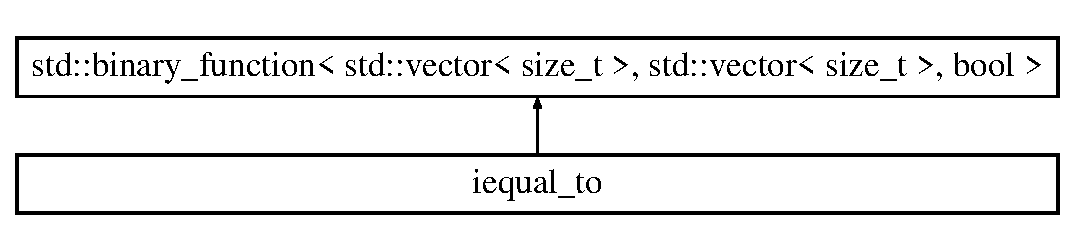
\includegraphics[height=2.000000cm]{structiequal__to}
\end{center}
\end{figure}
\subsection*{Public Member Functions}
\begin{DoxyCompactItemize}
\item 
\hypertarget{structiequal__to_a30c517fd40309fbd7f76ed1abc625717}{bool {\bfseries operator()} (std\-::vector$<$ size\-\_\-t $>$ const \&x, std\-::vector$<$ size\-\_\-t $>$ const \&y) const }\label{structiequal__to_a30c517fd40309fbd7f76ed1abc625717}

\end{DoxyCompactItemize}


The documentation for this struct was generated from the following file\-:\begin{DoxyCompactItemize}
\item 
Lifted\-L\-P\-Wrapper.\-hpp\end{DoxyCompactItemize}

\hypertarget{structihash}{\section{ihash Struct Reference}
\label{structihash}\index{ihash@{ihash}}
}
Inheritance diagram for ihash\-:\begin{figure}[H]
\begin{center}
\leavevmode
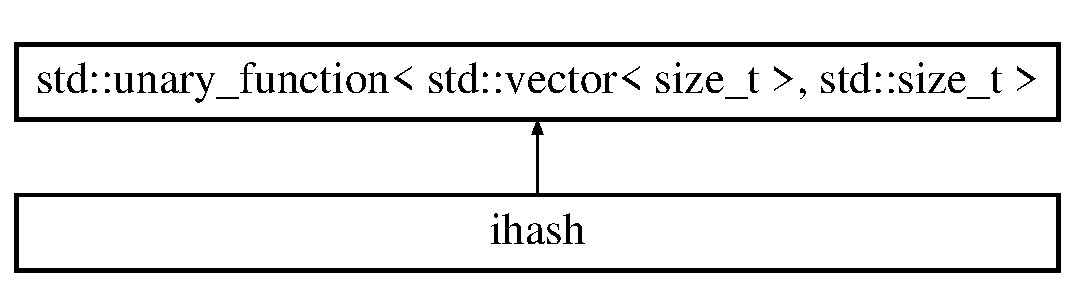
\includegraphics[height=2.000000cm]{structihash}
\end{center}
\end{figure}
\subsection*{Public Member Functions}
\begin{DoxyCompactItemize}
\item 
\hypertarget{structihash_aee085581d64eaa4ffb8547512d1da2fc}{std\-::size\-\_\-t {\bfseries operator()} (std\-::vector$<$ size\-\_\-t $>$ const \&x) const }\label{structihash_aee085581d64eaa4ffb8547512d1da2fc}

\end{DoxyCompactItemize}


The documentation for this struct was generated from the following file\-:\begin{DoxyCompactItemize}
\item 
Lifted\-L\-P\-Wrapper.\-hpp\end{DoxyCompactItemize}

\hypertarget{structoption}{\section{option Struct Reference}
\label{structoption}\index{option@{option}}
}
\subsection*{Public Attributes}
\begin{DoxyCompactItemize}
\item 
\hypertarget{structoption_a92c850a23c7828c1dba453bf8d15e1f0}{char $\ast$ {\bfseries name}}\label{structoption_a92c850a23c7828c1dba453bf8d15e1f0}

\item 
\hypertarget{structoption_a27b8e131fd56fbd4af053ca4692bedfe}{char {\bfseries letter}}\label{structoption_a27b8e131fd56fbd4af053ca4692bedfe}

\item 
\hypertarget{structoption_ab0a1bafa951008959d848d917a709f06}{char $\ast$ {\bfseries argname}}\label{structoption_ab0a1bafa951008959d848d917a709f06}

\item 
\hypertarget{structoption_a7c54cd6e10438ef77f481826160e41d8}{void($\ast$ {\bfseries callback} )(char $\ast$)}\label{structoption_a7c54cd6e10438ef77f481826160e41d8}

\item 
\hypertarget{structoption_a957577e49cd153ae34d79d57662436da}{char $\ast$ {\bfseries description}}\label{structoption_a957577e49cd153ae34d79d57662436da}

\end{DoxyCompactItemize}


The documentation for this struct was generated from the following file\-:\begin{DoxyCompactItemize}
\item 
util.\-h\end{DoxyCompactItemize}

\hypertarget{structsaucy}{\section{saucy Struct Reference}
\label{structsaucy}\index{saucy@{saucy}}
}
\subsection*{Public Attributes}
\begin{DoxyCompactItemize}
\item 
\hypertarget{structsaucy_a2ad14918933588cfb33f2801cdf9cd80}{int {\bfseries n}}\label{structsaucy_a2ad14918933588cfb33f2801cdf9cd80}

\item 
\hypertarget{structsaucy_a58b37ec8ebb0319e7963ed78bdfdc950}{const int $\ast$ {\bfseries adj}}\label{structsaucy_a58b37ec8ebb0319e7963ed78bdfdc950}

\item 
\hypertarget{structsaucy_a05c6221f65c09c8a01edcd4cf9e26624}{const int $\ast$ {\bfseries edg}}\label{structsaucy_a05c6221f65c09c8a01edcd4cf9e26624}

\item 
\hypertarget{structsaucy_ad0b4ddb844311a0ae73c7435c1d803f1}{const int $\ast$ {\bfseries dadj}}\label{structsaucy_ad0b4ddb844311a0ae73c7435c1d803f1}

\item 
\hypertarget{structsaucy_a7d86a99242cdc3f7fc07ec381073f464}{const int $\ast$ {\bfseries dedg}}\label{structsaucy_a7d86a99242cdc3f7fc07ec381073f464}

\item 
\hypertarget{structsaucy_a3e93870fe022773d46674916a72fb0fc}{void $\ast$ {\bfseries arg}}\label{structsaucy_a3e93870fe022773d46674916a72fb0fc}

\item 
\hypertarget{structsaucy_a626627bbf2fcb33c7b83c311e2b59362}{struct \hyperlink{structcoloring}{coloring} left {\bfseries right}}\label{structsaucy_a626627bbf2fcb33c7b83c311e2b59362}

\item 
\hypertarget{structsaucy_a1bdf0eb3fa08a7ef9b4656db5d15862d}{int $\ast$ {\bfseries nextnon}}\label{structsaucy_a1bdf0eb3fa08a7ef9b4656db5d15862d}

\item 
\hypertarget{structsaucy_a720b38e00ab5ae56d196222fc7c3f5da}{int $\ast$ {\bfseries prevnon}}\label{structsaucy_a720b38e00ab5ae56d196222fc7c3f5da}

\item 
\hypertarget{structsaucy_af529ff7df462f0476eb33a8320dd15a5}{char $\ast$ {\bfseries indmark}}\label{structsaucy_af529ff7df462f0476eb33a8320dd15a5}

\item 
\hypertarget{structsaucy_a0af5f7600ccb5f9bbdd709c921a79c62}{int $\ast$ {\bfseries ninduce}}\label{structsaucy_a0af5f7600ccb5f9bbdd709c921a79c62}

\item 
\hypertarget{structsaucy_a17e292d78b64853b9d116c8c29b40e52}{int $\ast$ {\bfseries sinduce}}\label{structsaucy_a17e292d78b64853b9d116c8c29b40e52}

\item 
\hypertarget{structsaucy_ad54fde58cd6a57422b63070f5734e78a}{int {\bfseries nninduce}}\label{structsaucy_ad54fde58cd6a57422b63070f5734e78a}

\item 
\hypertarget{structsaucy_a90f2f4bf21e76e3e9e1de1d5e36453d3}{int {\bfseries nsinduce}}\label{structsaucy_a90f2f4bf21e76e3e9e1de1d5e36453d3}

\item 
\hypertarget{structsaucy_a5e714ed5fb17929320c9eb7427bfc8ee}{int $\ast$ {\bfseries clist}}\label{structsaucy_a5e714ed5fb17929320c9eb7427bfc8ee}

\item 
\hypertarget{structsaucy_a3eeccf1aeb551130160a36f485390332}{int {\bfseries csize}}\label{structsaucy_a3eeccf1aeb551130160a36f485390332}

\item 
\hypertarget{structsaucy_a8c26da6f6430786f0f8d78cc807ae059}{char $\ast$ {\bfseries stuff}}\label{structsaucy_a8c26da6f6430786f0f8d78cc807ae059}

\item 
\hypertarget{structsaucy_ae202ba1235d09a03609925ca02353f13}{int $\ast$ {\bfseries ccount}}\label{structsaucy_ae202ba1235d09a03609925ca02353f13}

\item 
\hypertarget{structsaucy_ae1a027e42d895a469ec76442f6e46075}{int $\ast$ {\bfseries bucket}}\label{structsaucy_ae1a027e42d895a469ec76442f6e46075}

\item 
\hypertarget{structsaucy_a7fd586025ad878a3045e10f45f19f236}{int $\ast$ {\bfseries count}}\label{structsaucy_a7fd586025ad878a3045e10f45f19f236}

\item 
\hypertarget{structsaucy_aae66e06fd37cd0e163eb4791b67e46dd}{int $\ast$ {\bfseries junk}}\label{structsaucy_aae66e06fd37cd0e163eb4791b67e46dd}

\item 
\hypertarget{structsaucy_a700992de7bed66411fde1572661c6334}{int $\ast$ {\bfseries gamma}}\label{structsaucy_a700992de7bed66411fde1572661c6334}

\item 
\hypertarget{structsaucy_a2dab0e27910b6a4b7af7aae1ae5b835b}{int $\ast$ {\bfseries conncnts}}\label{structsaucy_a2dab0e27910b6a4b7af7aae1ae5b835b}

\item 
\hypertarget{structsaucy_a2f2fb9060babaf4bf77e60052f51e474}{int {\bfseries lev}}\label{structsaucy_a2f2fb9060babaf4bf77e60052f51e474}

\item 
\hypertarget{structsaucy_a6bf5ac5af61e5dc31cf3be6e276b24be}{int {\bfseries anc}}\label{structsaucy_a6bf5ac5af61e5dc31cf3be6e276b24be}

\item 
\hypertarget{structsaucy_a2f112a2294c870782379432326485f44}{int $\ast$ {\bfseries anctar}}\label{structsaucy_a2f112a2294c870782379432326485f44}

\item 
\hypertarget{structsaucy_a1e4a47f69660742b0f3081f5e7409340}{int {\bfseries kanctar}}\label{structsaucy_a1e4a47f69660742b0f3081f5e7409340}

\item 
\hypertarget{structsaucy_ab735de26f15bd1b42d5f087c1c6f6899}{int $\ast$ {\bfseries start}}\label{structsaucy_ab735de26f15bd1b42d5f087c1c6f6899}

\item 
\hypertarget{structsaucy_a4b2a6dc8ca8b9697c5c6e3c560b51f58}{int {\bfseries indmin}}\label{structsaucy_a4b2a6dc8ca8b9697c5c6e3c560b51f58}

\item 
\hypertarget{structsaucy_a7d2723440200df0ab62b3b521d52a1b6}{int {\bfseries match}}\label{structsaucy_a7d2723440200df0ab62b3b521d52a1b6}

\item 
\hypertarget{structsaucy_a533be1a3b6c1d6c3e70253f77062df26}{int $\ast$ {\bfseries theta}}\label{structsaucy_a533be1a3b6c1d6c3e70253f77062df26}

\item 
\hypertarget{structsaucy_a7c75f93b21378ca6e2fbaca635987ae4}{int $\ast$ {\bfseries thsize}}\label{structsaucy_a7c75f93b21378ca6e2fbaca635987ae4}

\item 
\hypertarget{structsaucy_a8066648db0b6019242e1c1fd789a93a4}{int $\ast$ {\bfseries thnext}}\label{structsaucy_a8066648db0b6019242e1c1fd789a93a4}

\item 
\hypertarget{structsaucy_a6d033ed9e5ccbd72e2776be38b64ce7c}{int $\ast$ {\bfseries thprev}}\label{structsaucy_a6d033ed9e5ccbd72e2776be38b64ce7c}

\item 
\hypertarget{structsaucy_a618009662eb7972ea332e85dd62fff3f}{int $\ast$ {\bfseries threp}}\label{structsaucy_a618009662eb7972ea332e85dd62fff3f}

\item 
\hypertarget{structsaucy_ab1f355182f4d4c0447785eb753afd1b0}{int $\ast$ {\bfseries thfront}}\label{structsaucy_ab1f355182f4d4c0447785eb753afd1b0}

\item 
\hypertarget{structsaucy_a34d3675809b2b1a37dd274e447be48e4}{int $\ast$ {\bfseries splitwho}}\label{structsaucy_a34d3675809b2b1a37dd274e447be48e4}

\item 
\hypertarget{structsaucy_ab0ac0e70f85e4778205c76fba0bcb02c}{int $\ast$ {\bfseries splitfrom}}\label{structsaucy_ab0ac0e70f85e4778205c76fba0bcb02c}

\item 
\hypertarget{structsaucy_a22c74ce29ad86980b079fe5925128d93}{int $\ast$ {\bfseries splitlev}}\label{structsaucy_a22c74ce29ad86980b079fe5925128d93}

\item 
\hypertarget{structsaucy_a3ce4eb3861c1e1d1c348aa182ea1f333}{int {\bfseries nsplits}}\label{structsaucy_a3ce4eb3861c1e1d1c348aa182ea1f333}

\item 
\hypertarget{structsaucy_a7affcdc76251a0ccd0eb616efc6c1c05}{char $\ast$ {\bfseries diffmark}}\label{structsaucy_a7affcdc76251a0ccd0eb616efc6c1c05}

\item 
\hypertarget{structsaucy_aa3d5bdb5a31322669a22f535c6e1755f}{int $\ast$ {\bfseries diffs}}\label{structsaucy_aa3d5bdb5a31322669a22f535c6e1755f}

\item 
\hypertarget{structsaucy_afee75913d84db04b1cfdc182856aa09d}{int $\ast$ {\bfseries difflev}}\label{structsaucy_afee75913d84db04b1cfdc182856aa09d}

\item 
\hypertarget{structsaucy_aae0f7e1a0560056bb3532c4a4a95b49f}{int {\bfseries ndiffs}}\label{structsaucy_aae0f7e1a0560056bb3532c4a4a95b49f}

\item 
\hypertarget{structsaucy_a4ab576921e083a2a80583e16cafab0a3}{int $\ast$ {\bfseries undifflev}}\label{structsaucy_a4ab576921e083a2a80583e16cafab0a3}

\item 
\hypertarget{structsaucy_a4a5657437a366285ab7302af13f11337}{int {\bfseries nundiffs}}\label{structsaucy_a4a5657437a366285ab7302af13f11337}

\item 
\hypertarget{structsaucy_ac5a3a0a80030d62b99f27eed17a57e2d}{int $\ast$ {\bfseries unsupp}}\label{structsaucy_ac5a3a0a80030d62b99f27eed17a57e2d}

\item 
\hypertarget{structsaucy_a723aaac76801f8718669622bb54bba82}{int $\ast$ {\bfseries specmin}}\label{structsaucy_a723aaac76801f8718669622bb54bba82}

\item 
\hypertarget{structsaucy_abec9435324752b5bcb02cbe82a31bd1e}{int $\ast$ {\bfseries pairs}}\label{structsaucy_abec9435324752b5bcb02cbe82a31bd1e}

\item 
\hypertarget{structsaucy_af4815e969a73e5e0210068d69371bad8}{int $\ast$ {\bfseries unpairs}}\label{structsaucy_af4815e969a73e5e0210068d69371bad8}

\item 
\hypertarget{structsaucy_a43e8bf7f7c1fa38167f3fd5d7aa1d974}{int {\bfseries npairs}}\label{structsaucy_a43e8bf7f7c1fa38167f3fd5d7aa1d974}

\item 
\hypertarget{structsaucy_ad9760ae6db39a88fb57e6eb6697a5e55}{int $\ast$ {\bfseries diffnons}}\label{structsaucy_ad9760ae6db39a88fb57e6eb6697a5e55}

\item 
\hypertarget{structsaucy_a6cef198aa1be5fda2af744166cb394a6}{int $\ast$ {\bfseries undiffnons}}\label{structsaucy_a6cef198aa1be5fda2af744166cb394a6}

\item 
\hypertarget{structsaucy_a88dfe33adfdb28e3d63e3c5463445baa}{int {\bfseries ndiffnons}}\label{structsaucy_a88dfe33adfdb28e3d63e3c5463445baa}

\item 
\hypertarget{structsaucy_ad2aa284e5cbd5353db3aa350d2c8478a}{saucy\-\_\-consumer $\ast$ {\bfseries consumer}}\label{structsaucy_ad2aa284e5cbd5353db3aa350d2c8478a}

\item 
\hypertarget{structsaucy_a3b73cc72ca8f102ff4b5149df0e38855}{int($\ast$ {\bfseries split} )(struct \hyperlink{structsaucy}{saucy} $\ast$, struct \hyperlink{structcoloring}{coloring} $\ast$, int, int)}\label{structsaucy_a3b73cc72ca8f102ff4b5149df0e38855}

\item 
\hypertarget{structsaucy_a70c592b2d42e48246ee1b81b5dde9250}{int($\ast$ {\bfseries is\-\_\-automorphism} )(struct \hyperlink{structsaucy}{saucy} $\ast$)}\label{structsaucy_a70c592b2d42e48246ee1b81b5dde9250}

\item 
\hypertarget{structsaucy_aebd7e4479e6757ba8c63bf09813838b5}{int($\ast$ {\bfseries ref\-\_\-singleton} )(struct \hyperlink{structsaucy}{saucy} $\ast$, struct \hyperlink{structcoloring}{coloring} $\ast$, int)}\label{structsaucy_aebd7e4479e6757ba8c63bf09813838b5}

\item 
\hypertarget{structsaucy_a104924cb7e33331b40451bbdd6f9f151}{int($\ast$ {\bfseries ref\-\_\-nonsingle} )(struct \hyperlink{structsaucy}{saucy} $\ast$, struct \hyperlink{structcoloring}{coloring} $\ast$, int)}\label{structsaucy_a104924cb7e33331b40451bbdd6f9f151}

\item 
\hypertarget{structsaucy_a3a8e6e9aa0f769b28a1a646937a077e0}{struct \hyperlink{structsaucy__stats}{saucy\-\_\-stats} $\ast$ {\bfseries stats}}\label{structsaucy_a3a8e6e9aa0f769b28a1a646937a077e0}

\end{DoxyCompactItemize}


The documentation for this struct was generated from the following file\-:\begin{DoxyCompactItemize}
\item 
saucy.\-c\end{DoxyCompactItemize}

\hypertarget{structsaucy__graph}{\section{saucy\-\_\-graph Struct Reference}
\label{structsaucy__graph}\index{saucy\-\_\-graph@{saucy\-\_\-graph}}
}
\subsection*{Public Attributes}
\begin{DoxyCompactItemize}
\item 
\hypertarget{structsaucy__graph_afeb103fea03d7425bc29f286017e1050}{int {\bfseries n}}\label{structsaucy__graph_afeb103fea03d7425bc29f286017e1050}

\item 
\hypertarget{structsaucy__graph_a42d7a4a649a18c85740ec2b03c51762f}{int {\bfseries e}}\label{structsaucy__graph_a42d7a4a649a18c85740ec2b03c51762f}

\item 
\hypertarget{structsaucy__graph_aa19c0d5222c0281f25757befd6fcaa4c}{int $\ast$ {\bfseries adj}}\label{structsaucy__graph_aa19c0d5222c0281f25757befd6fcaa4c}

\item 
\hypertarget{structsaucy__graph_aee3c06170c9790cc78d4035a28c919a3}{int $\ast$ {\bfseries edg}}\label{structsaucy__graph_aee3c06170c9790cc78d4035a28c919a3}

\end{DoxyCompactItemize}


The documentation for this struct was generated from the following file\-:\begin{DoxyCompactItemize}
\item 
saucy.\-h\end{DoxyCompactItemize}

\hypertarget{structsaucy__stats}{\section{saucy\-\_\-stats Struct Reference}
\label{structsaucy__stats}\index{saucy\-\_\-stats@{saucy\-\_\-stats}}
}
\subsection*{Public Attributes}
\begin{DoxyCompactItemize}
\item 
\hypertarget{structsaucy__stats_a1df2b4661fe674b4f41e6b74c757c4b7}{double {\bfseries grpsize\-\_\-base}}\label{structsaucy__stats_a1df2b4661fe674b4f41e6b74c757c4b7}

\item 
\hypertarget{structsaucy__stats_a1e439c519ef94116148ebed5896cb82c}{int {\bfseries grpsize\-\_\-exp}}\label{structsaucy__stats_a1e439c519ef94116148ebed5896cb82c}

\item 
\hypertarget{structsaucy__stats_ac07b88469b78ff40586b7149ccc8da5f}{int {\bfseries levels}}\label{structsaucy__stats_ac07b88469b78ff40586b7149ccc8da5f}

\item 
\hypertarget{structsaucy__stats_a0f30ed579f785dda0ca067866ef960cc}{int {\bfseries nodes}}\label{structsaucy__stats_a0f30ed579f785dda0ca067866ef960cc}

\item 
\hypertarget{structsaucy__stats_a158aee6bf48f81cc3ad1748670f6d91f}{int {\bfseries bads}}\label{structsaucy__stats_a158aee6bf48f81cc3ad1748670f6d91f}

\item 
\hypertarget{structsaucy__stats_a1526f378811c0bb2e48ed70743d5f078}{int {\bfseries gens}}\label{structsaucy__stats_a1526f378811c0bb2e48ed70743d5f078}

\item 
\hypertarget{structsaucy__stats_a7723003bb9d8ec737413fbd46b17a2ea}{int {\bfseries support}}\label{structsaucy__stats_a7723003bb9d8ec737413fbd46b17a2ea}

\end{DoxyCompactItemize}


The documentation for this struct was generated from the following file\-:\begin{DoxyCompactItemize}
\item 
saucy.\-h\end{DoxyCompactItemize}

\hypertarget{classsorter}{\section{sorter$<$ T $>$ Class Template Reference}
\label{classsorter}\index{sorter$<$ T $>$@{sorter$<$ T $>$}}
}
\subsection*{Public Member Functions}
\begin{DoxyCompactItemize}
\item 
\hypertarget{classsorter_abb8ae32e511bdb671a138edac6d34242}{{\bfseries sorter} (const std\-::vector$<$ T $>$ \&v)}\label{classsorter_abb8ae32e511bdb671a138edac6d34242}

\item 
\hypertarget{classsorter_aa9f76153f9ed38a9c1f808b224e0f0ae}{bool {\bfseries operator()} (int a, int b)}\label{classsorter_aa9f76153f9ed38a9c1f808b224e0f0ae}

\end{DoxyCompactItemize}


The documentation for this class was generated from the following file\-:\begin{DoxyCompactItemize}
\item 
W\-L.\-cpp\end{DoxyCompactItemize}

%--- End generated contents ---

% Index
\newpage
\phantomsection
\addcontentsline{toc}{chapter}{Index}
\printindex

\end{document}
